
\section{Applications and Experiments}


We show broad applications of the proposed RL text generation framework to a variety of problems where no clean supervision data is available. These include learning with noisy or even negative data (\S\ref{subsec:noisy-data}), generating adversarial text attacks (\S\ref{subsec:adversarial-attack}), and generating prompts to steer pretrained LMs (\S\ref{subsec:prompt-generation}).
We also study the performance on standard supervised generation tasks (\S\ref{appendix-subsec:standard-tasks}) and show that our approach is competitive to train text generation models \emph{from scratch}. We provide detailed configurations in the appendix (\S\ref{appendix-subsec:setup-details}).

\subsection{Learning from Noisy (Negative) Text}
\label{subsec:noisy-data}

The popular MLE algorithm learns by (blindly) imitating training data.
However,
it is often expensive to curate clean quality data. It is thus highly desirable to be able to learn from data with noises, or even \emph{negative} examples.
With the guidance of task metrics (rewards), the model can even learn to ``outperform'' the training data and achieve desired generation behaviors.
To this end, we consider the task of \emph{entailment generation}~\citep{pasunuru2017multi}. Given a sentence (premise), the goal is to generate a new sentence (hypothesis) that logically follows the premise. 



\begin{figure*}
    \centering
    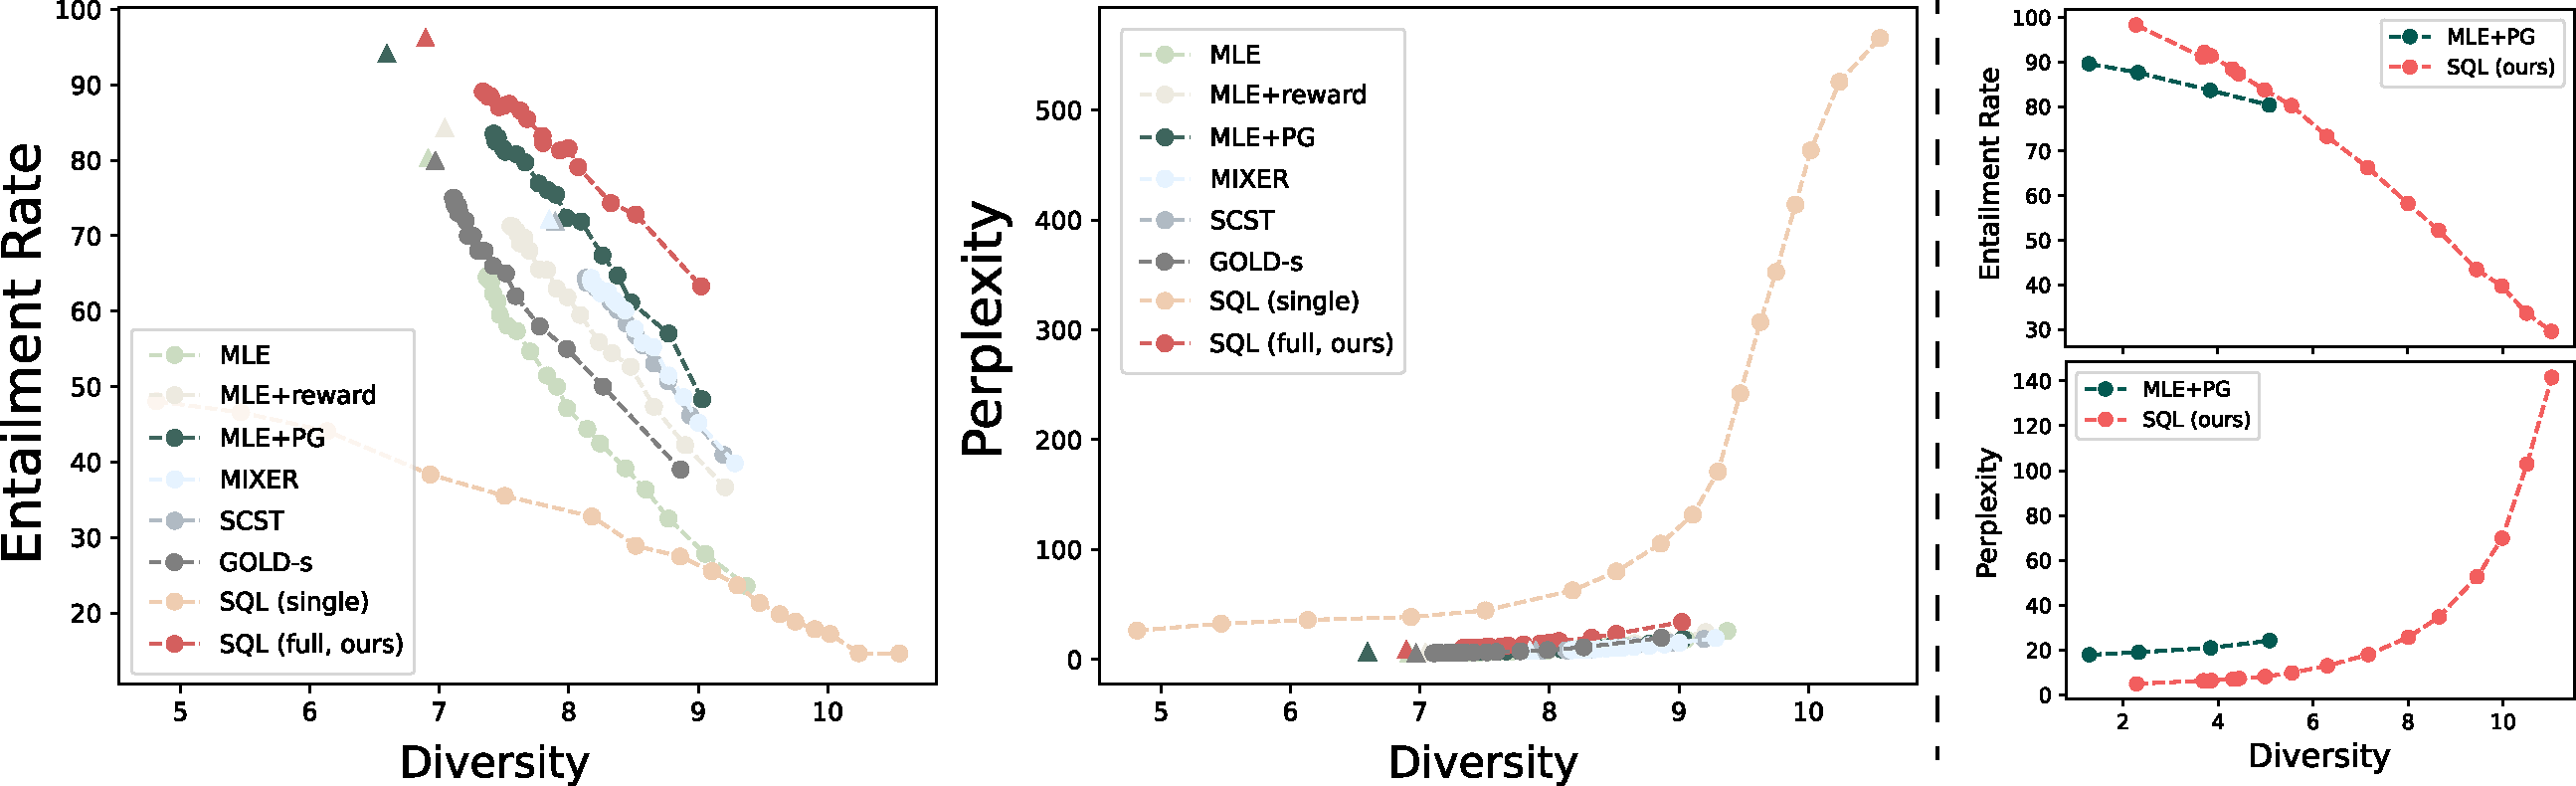
\includegraphics[width=0.99\linewidth]{figures/202101005-entailment-combined.pdf}
    \vspace{-7pt}
    \caption{
    \textbf{Left:} entailment generation performance plotted against diversity (average of $H_1$ and $H_2$). 
    Circles represent results of top-$p$ sample outputs,
    and triangles represent results of beam-search outputs.
    Please see Table~\ref{table:entailment-generation} for additional results.
    \textbf{Right:} entailment attack performance against diversity. 
    Only a few \texttt{MLE+PG} dots are visible because the model is not able to generate more diverse samples even with increasing $p$ value in top-$p$ decoding, i.e., the model collapses.
    }
    \label{fig:entailment-generation}
    \label{fig:entailment-attack}
    \vspace{-5pt}
\end{figure*}


\paragraph{Setup (more in~\S\ref{appendix-subsubsec:setup-noisy-data}).}
We sub-sampled $50k$ training examples from the SNLI dataset~\citep{bowman2015large}, a commonly used entailment classification dataset. The hypotheses have an average entailment probability of only $50\%$, and over $2/5$ of them less than $20\%$ (negative/contradictive examples) -- a significant challenge for the models to learn from the noises. 
The rewards include (1) the entailment score of the generation measured by a robust entailment classifier~\citep{nie2020adversarial}, (2) the log-likelihood of the generation as an indicator of language quality measured by a GPT-2 language model~\citep{radford2019language}, and (3) BLEU score w.r.t the input premises as another language quality reward that avoids trivial outputs. We sum together all rewards with weights $1.0$.

We compare our approach with a broad range of baselines, including 
(1) the standard MLE training (\texttt{MLE}); 
(2) \texttt{MLE+reward}, where we use the reward function to filter examples;
(3) joint MLE and PG training with MLE initialization (\texttt{MLE+PG}), where we initialize the model with MLE training, then train it with combined MLE and PG losses;
previous text-generation RL algorithms including (4) \texttt{MIXER}~\citep{ranzato2015sequence}, 
(5) \texttt{Self-critic}~\citep{rennie2017self}, 
and 
(6) one of the latest methods \texttt{GOLD-$s$}~\citep{pang2021text} which is a pure off-policy method based on importance-sampling PG. 
To ablate the effect of multi-step training (\S\ref{subsec:method:pcl}), we additionally compare with a simplified variant of our approach that uses only vanilla single-step PCL training (\texttt{SQL(single)}). We include more baselines such as MLE weighted by rewards in \S\ref{appendix-subsubsec:experiments-noisy-data}.




We evaluate generation results in terms of entailment rate, language quality (perplexity), and diversity which is measured by the Shannon entropy over unigrams and bigrams ($H_1$, $H_2$) \citep{gehrmann2021gem}. Since text generation models intrinsically
trade off diversity and quality \citep{caccia2019language,hashimoto2019unifying}, we vary the generation diversity by generating samples via top-$p$ sampling \citep{holtzman2019curious} with different $p$ values, and plot the entailment rate and perplexity against diversity, resp. We also evaluate the samples produced by beam-search decoding.

\paragraph{Results.}
Figure~\ref{fig:entailment-generation} (left) shows the results, and Table~\ref{table:entailment-generation-examples-sql} shows samples.
First, notice that \texttt{MLE} performs poorly, while \texttt{MLE+reward} improves upon it. This is not surprising as the training data contain noisy/negative examples. Similarly, since the pure off-policy algorithm \texttt{GOLD-$s$} relies heavily on the data distribution, we observed that it achieves sub-optimal performance. The on-policy \texttt{MLE+PG} with MLE initialization gives better entailment rate.
In comparison, our full \texttt{SQL} framework achieves the best entailment-diversity trade-off. 
The comparison between \texttt{SQL} and \texttt{SQL(single)} highlights the importance of having the multi-step objective which directly uses the end reward rather than bootstrapping intermediate $Q$-values for supervision.



















\subsection{\textit{Universal} Adversarial Attacks}
\label{subsec:adversarial-attack}

We next study the application
in text adversarial attacks, where again no supervised data is available. 
Adversarial attacks is an increasingly important research topic as they reveal models' vulnerabilities and flaws. This is especially true for universal attacks~\citep{wallace2019universal,atanasova2020generating}, where we want to generate universal examples that trick the model on \emph{all} possible inputs. 
For instance, consider the context of entailment classification.
Our goal is to find universal human-readable hypotheses that are going to be classified as ``entailment'' with as high probability as possible, regardless of the input premises. This is a more challenging setting compared to previous instance-specific attack \citep{morris2020textattack,jin2020bert,ebrahimi2017hotflip} where the attack model conditions on a premise and generates an adversarial hypothesis specific to the premise. 


\paragraph{Setup (more in~\S\ref{appendix-subsubsec:setup-adversarial-attack}).}
We aim to attack one of the most popular MultiNLI~\citep{williams2018broad} entailment classifiers on HuggingFaceHub.\footnote{\url{https://github.com/pytorch/fairseq/tree/master/examples/roberta}
} The attack generation model generates adversarial text without conditioning on any inputs so that the generated attacks are universal to all premises.  
We compare our \texttt{SQL} with \texttt{MLE+PG}. We use all hypotheses in the MultiNLI dataset as the training data for the MLE training in \texttt{MLE+PG} and the off-policy updates for our \texttt{SQL}.
We do not compare with previous specialized adversarial text attack methods, because they either are not applicable to the challenging universal attack setting \citep{morris2020textattack,jin2020bert,ebrahimi2017hotflip}, or were not designed to generate human-readable sentences \citep{wallace2019universal}. 
We use similar settings as in \S\ref{subsec:noisy-data} to explore the diversity-quality trade-off 
by plotting the entailment rate and perplexity against diversity, respectively. 
The entailment classifier to be attacked is used as entailment score reward functions. We also include a token-level repetition penalty reward for readability.


\paragraph{Results.}

Figure~\ref{fig:entailment-attack} (right) shows the results, and Table~\ref{table:entailment-attack-examples} shows samples.
We can see that \texttt{SQL} outperforms \texttt{MLE+PG} consistently across different diversity values. The outputs from \texttt{MLE+PG} are not diverse even with high $p$'s, indicating the model collapses and can only generate a small set of unique adversarial examples. 
The model by \texttt{SQL} discovers the pattern ``saint-pierre-et-saint-paul'' (an entity name), and exploits this to generate samples with high universal entailment rate.


\begin{figure}[t]
    \centering
    \begin{minipage}{.49\textwidth}
        \centering
        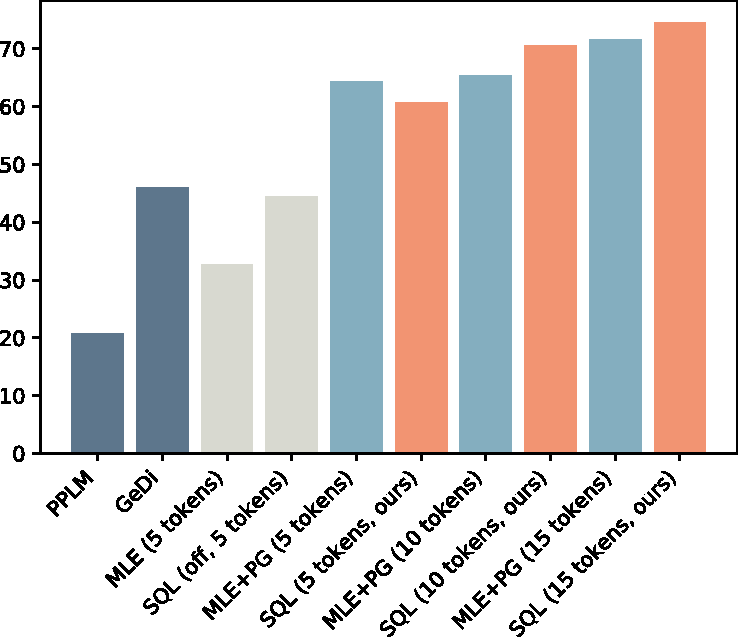
\includegraphics[width=0.75\linewidth]{figures/20210527.prompt-generation.pdf}
        \vspace{-7pt}
        \caption{Average topic accuracy. Please see Table~\ref{table:prompt-generation-full} for more details.}
        \label{fig:prompt-generation-topic}
\end{minipage}%
\hfill
\begin{minipage}{0.49\textwidth}
\centering
\small
\begin{tabular}{@{}llll@{}}
\toprule
\textbf{PPLM} & \textbf{GeDi} & \textbf{MLE (5)} & \textbf{SQL (off, 5)} \\
\midrule
$13.07$ & $123.88$ & $25.70$ & $25.77$ \\
\midrule
\multicolumn{2}{l}{\textbf{MLE+PG (5/10/15)}} & \multicolumn{2}{l}{\textbf{SQL (5/10/15, ours)}} \\
\midrule
\multicolumn{2}{l}{$25.52$/$28.16$/$28.71$} & \multicolumn{2}{l}{$25.94$/$26.95$/$29.10$} \\
\bottomrule
\end{tabular}
\vspace{-7pt}
\captionof{table}{
Average perplexity across topics. The lower, the more fluent the generated continuation sentences.
}
\vspace{-5pt}
\label{table:prompt-generation}

\vspace{9pt}

\centering
\small
\begin{tabular}{p{0.79cm}p{0.6cm}p{0.6cm}p{0.6cm}}
\toprule
\textbf{Model} & PPLM & GeDi & SQL \\
\midrule
\textbf{Seconds} & $5.58$ & $1.05$ & $0.07$ \\
\bottomrule
\end{tabular}
\vspace{-7pt}
\caption{Average sentence generation time cost.}
\vspace{-7pt}
\label{table:prompt-generation-speed}
\end{minipage}
\vspace{-7pt}
\end{figure}


\subsection{Prompt Generation for Controlling Pretrained Language Models}
\label{subsec:prompt-generation}





A reward function does not just have to be a metric like the BLEU score, but also a complicated pipeline that eventually returns a score.
To demonstrate this, we consider the emerging task of prompting a large pretrained LM for controllable generation \citep{Hu2017TowardCG,radford2019language,NEURIPS2020_1457c0d6}.
The goal is to learn to generate text prompts that steer the LM to generate sentences of certain desired attributes (e.g., topics). 
The problem of controlling the generation of pretrained LMs was previously approached through specialized algorithms such as modifying the LM hidden states during decoding~\citep{Dathathri2020Plug,krause2020gedi,qin2020backpropagation}. Here we show that prompts offer an easier, faster, more effective way for controlled generation.

Learning to generate/tune prompts is gaining increasing attention recently.
It side-steps the needs for expensive LM fine-tuning, and adapts LMs to new scenarios with prompt as the (compute-friendly) interface.
Most existing approaches~\citep{wallace2019universal,li2021prefix,lester2021power} rely on gradient backpropagation and are applicable only when the whole training pipeline is differentiable.
This does not hold for the text generation setting, as illustrated in Figure~\ref{fig:prompt-generation-flow}. In contrast, the RL framework is generally applicable to any differentiable or discrete pipelines.


\begin{figure}
\centering
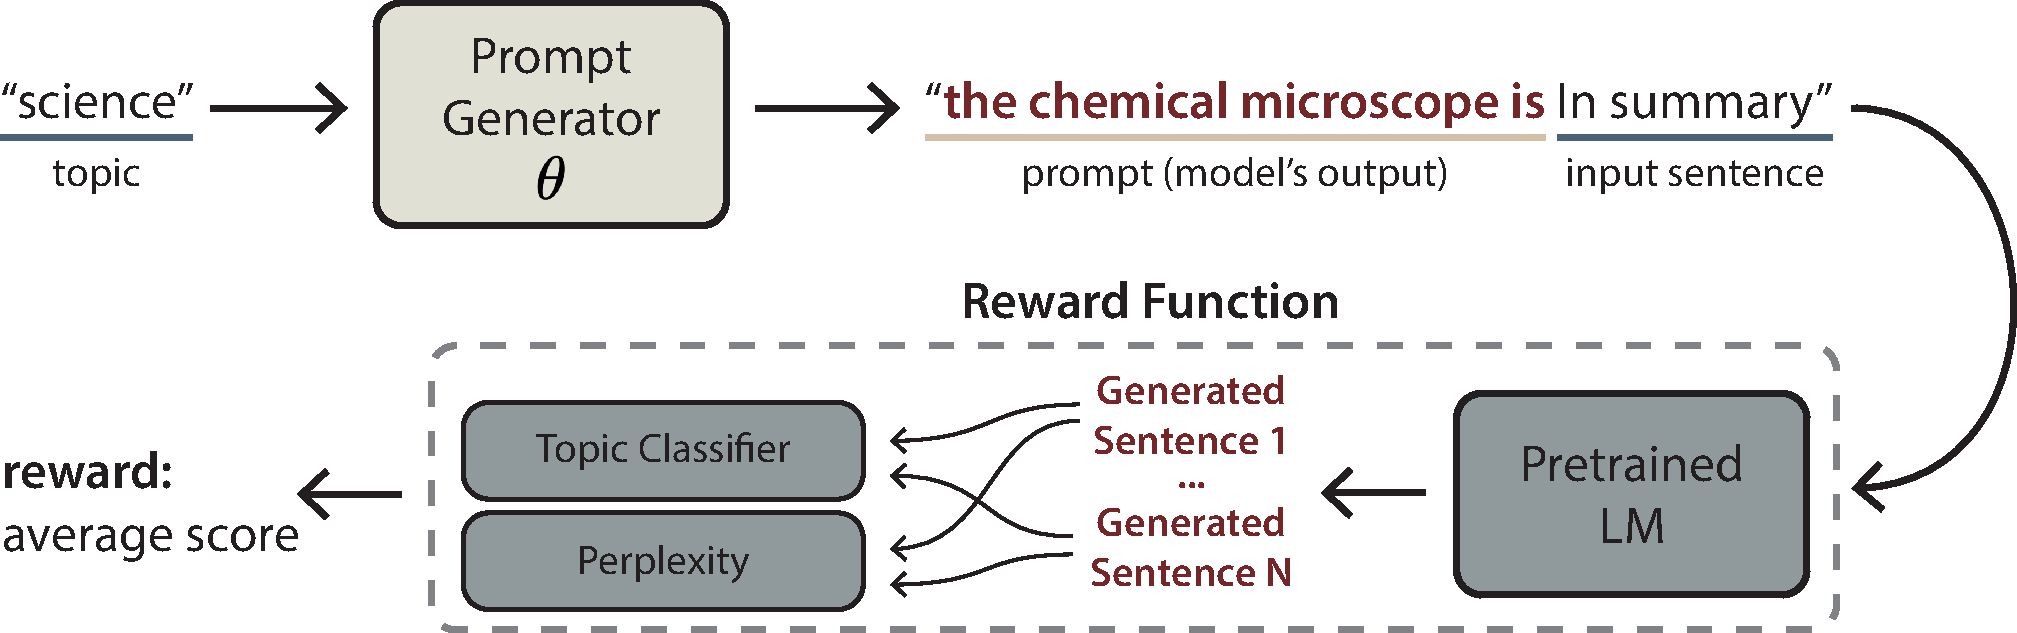
\includegraphics[width=0.99\linewidth]{figures/prompt-generation-task-new.pdf}
\vspace{-12pt}
\caption{
The scheme of prompt generation for controlling the outputs of pretraind LMs.
}
\vspace{-7pt}
\label{fig:prompt-generation-flow}
\end{figure}


\paragraph{Setup (more in~\S\ref{appendix-subsubsec:setup-prompt-generation}).}
Following \citep{dathathri2019plug}, we aim to control the generation to have one of 7 topics (e.g., ``science''); the generated prompt is prepended to one of 20 input sentences for the pretrained LM to generate continuation sentences. Figure~\ref{fig:prompt-generation-flow} shows the architecture of prompt-based controllable generation. We compare our \texttt{SQL} method with \texttt{MLE+PG} as before. Since the prompt length could impact the generated sentences, we conducted experiments with maximum prompt length $5$, $10$, and $15$. As ablation study, we also evaluate the SQL algorithm with only off-policy updates (i.e., without on-policy exploration), denoted as \texttt{SQL(off)}, and compare it with vanilla \texttt{MLE} training. Finally, we also compare with two specialized controllable generation techniques based on pretrained LMs, namely \texttt{PPLM}~\citep{dathathri2019plug} and \texttt{GeDi}~\citep{krause2020gedi}, following similar procedures using their open-sourced code. We use a distilled GPT-2 model\footnote{\url{https://huggingface.co/distilgpt2}} as the pretrained LM to be controlled. %
For rewards, we use the topic accuracy of the continuation sentences measured by a \emph{zero-shot} classifier, plus the the log-likelihood of continuation sentences as the language quality reward measured by a distilled GPT-2.\footnote{Note that the language quality emphasis is on the generated sentences. Prompts themselves do not necessarily have to be human-readable~\cite{wallace2019universal,sheng2020towards}.}


\paragraph{Results.}

Figure~\ref{fig:prompt-generation-topic} shows the topic accuracy of the controlled LM outputs averaged across the 7 topics, and Table~\ref{table:prompt-generation} shows the respective language quality results. More detailed topic accuracy results and samples are provided in the appendix (\S\ref{appendix-subsubsec:experiments-prompt-generation}) (where \texttt{GeDi} obtained low accuracy on 2 of the 7 topics, possibly because the topic tokens are tokenized into two subwords for which the model released by the authors was not specifically trained). 
We can see that the prompts generated by our \texttt{SQL} cause the LM to generate sentences with high topic accuracy while maintaining low perplexity in most settings.
Increasing the prompt length positively impacts the topic accuracy, which makes sense because longer prompts give more flexible for steering the LM.
The comparison between \texttt{MLE} and \texttt{SQL(off)}
shows that the off-policy component of SQL is better than standard MLE training, as it incorporates reward signals instead of just blindly following the (noisy) data. 

Next, comparing with the previous steered decoding such as \texttt{PPLM} and \texttt{GeDi},
we can see the prompt-based control trained with RL achieves better trade-off between topic accuracy and language quality. Moreover, once a prompt is produced, we can use the pretrained LM to generate text of desired topics efficiently, with the same time cost as standard non-controlled decoding. In comparison, the dedicated steered decoding is often orders-of-magnitude slower, as shown in Table~\ref{table:prompt-generation-speed}.





